\documentclass[main.tex]{subfiles} 
\begin{document}

\section*{Resultater}
\label{sec:4}

Å burke poengsum som vurderingskriterie for å vurdere elever var uheldig i denne sammenhengen siden jeg hadde vektlagt
de ''vanskelige`` oppgavene mye mer enn de ''enkle``. Nesten alle elever på tvers av nivå og ferdigheter hadde 
problemmer med å løse disse oppgavene og veldig få klarte å gå over en score på 5 ut av 10. Dermed fikk jeg ikke 
veldig mye informasjon om elevene gjennom poengsum. Oftest var det de faglige sterke i klassen som tangerte
mot 5 i poengsum. Ut ifra dette konkluderte jeg sammen med veileder at prøven var nok litt vanskeligere enn
det burde ha vært. Dessuten var det en deloppgave i prøven mange elever feiltolket, og her kan jeg godt
akseptere at det var lett å feiltolke hva oppgaven spør om :
\par
\begin{figure}[h!]
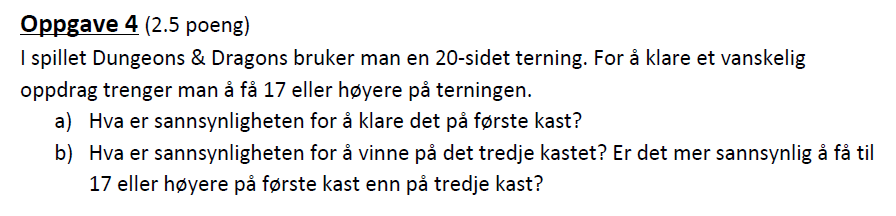
\includegraphics[scale = 0.7]{../figures/oppgave4b.png}
%\caption{Oversikt over naturfaglærernes undervisningstilbud til elevene fra PISA+ studie. Kilde: 
%\protect\citeA{odeg10}.}
%\label{fig:odeg10}
\end{figure}
I oppgave b står det \emph{Hva er sannsynligheten for å vinne på det tredje kastet?}. Her var hensikten at
elevene skulle oppfatte det som \emph{Hva er sannsynligheten for å tape på to runder på rad og deretter vinne på det tredje kastet?},
men mange oppfattet det som å vinne på tredje kastet uavhengig av hva som forekommer på de første to kast.
Dermed ville svaret til neste del av deloppgaven, \emph{Er det mer sannsynlig å få til 17 eller høyere på første kast enn
på det tredje kast?},  være ''like sannsynlig`` og det var ofte det elevene besvarte. Det var heller ikke hjelpsomt når 
denne oppgaven telte 15\% (dvs. 1.5 poeng) av hele prøven.  

finne og diskutere sannsyn gjennom eksperimentering, simulering og berekning i daglegdagse samanhengar og spel
beskrive utfallsrom og uttrykkje sannsyn som brøk, prosent og desimaltal


\end{document}
